%Implementierung_vollmatrize
Multiplikation von Matrize mit Vektor in CUDA Implementierung\\

Beim Wissenschaftlichen Rechen trifft man häufig die Multiplikation von Matritze mit Vektor. In CUDA Implementierung wird die Oparation als unterschiedliche Vektor-Multiplicationen zerlegt.Mit änlichem Methode werden auch Matizen mit Vektoren multipliziert. Im folgendem Bild Fig.\ref{MatrixVektor}.zeigt, dass jede zerlegte Vektor von A mit Vektor B in einem Block multipliziert wird. 

\begin{figure}[htbp]
%\centering
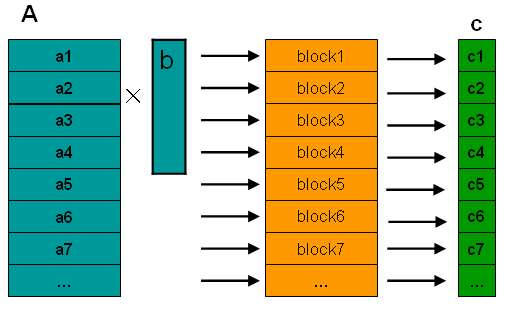
\includegraphics[width=3.5in]{.//pic//MatrixVektor}
\caption{Matrize mal Vektor. A: Matrize; b: Vektor; c: Produktvektor}
\label{MatrixVektor} 
\end{figure}